\documentclass{article}
\usepackage[T2A]{fontenc}

\hyphenation{ма-те-ма-ти-ка вос-ста-нав-ли-вать}
\usepackage[english, russian]{babel}
\usepackage{amsmath}
\usepackage{graphicx}
\graphicspath{ {./images/} }
\begin{document}
 
\tableofcontents

\section{Закон распределения простых чисел}

\paragraph{}
$\pi(x)$ -- Количество простых чисел, не превосходящих $x$.
Примерно равна интегралу:

\[ \pi(x) \approx Li(x) = \int_{2}^{x} \frac{1}{ln(t)} dt \approx \frac{x}{ln(x)} \]

Отсюда видно, что с ростом $x$ простые числа встречаются всё реже и реже.
Было найдено эмпирическим путём. Но доказано это было лишь спустя 100 лет.
Смысл в том, что:

\[ \lim_{x \to \infty} \frac{Li(x)}{\pi(x)} = \lim_{x \to \infty} \frac{x/ln(x)}{\pi(x)} = 1 \]

\section{Дзета-функция Римана}

\paragraph{}
Выглядит так:
\[ \zeta(s) = 1^{-s} + 2^{-s} + ... + n^{-s} \].

Похоже на ряд Тейлора, но наоборот. Сходится при $s > 1$ и расходится к бесконечности при s = 1
(получается гармонический ряд):

\[ \frac{1}{1} + \frac{1}{2} + \frac{1}{3} + .. + \frac{1}{n} + ... = \infty \]

\paragraph{}
Её изучал еще Эйлер. Он рассматривал похожую функцию --
\textbf{знакопеременную дзета-функцию}:

\[ \eta (s) = \sum_{1}^{\infty} (-1)^{n+1} n^{-s} = ... \]

Как они связаны?

\[ ... = (1 - 2 \times 2^{-s}) \zeta(s) \]

\paragraph{}
Если раскрыть скобки, то все чётные получается со знаком минус.
В чём соль? Этот ряд сходится при $s > 0$. Посчитаем ряд для $\eta$ функции и
поделим на это выражение. Таким образом мы доопределяем $\zeta$ функцию для чисел меньших 1.

\[ \eta(1) = \frac{1}{1} - \frac{1}{2} + .. + \frac{(-1)^{n+1}}{n} + ... = ln(2) \]

\section{Тождество Эйлера}

\paragraph{}
Эйлер дал новое определение для этой функции:

\[ \zeta(s) = \prod_{p - \text{простое}} \frac{1}{1 - p^{-s}} \]

\paragraph{}
Почему так получается? Заметим, что 

\[ \frac{1}{1 - p^{-s}} = 1 + \frac{1}{p^s} + \frac{1}{p^{2s}} + \frac{1}{p^{3s}} + ... \]

Что получится, если теперь в этом произведении раскрыть скобки?
Всевозможные произведения $p^s$ во всех степенях. По основной теореме арифметики
это даст нам в точности ряд для $\zeta$ функции.

\paragraph{}
В чём заключается применимость этого тождества?

\section{Доказательство бесконечности множестве простых чисел}

\paragraph{}
Это можно сделать и без тождества Эйлера, но с ним получается очень элегантно. Если бы количество простых чисел было конечным, то гармонический рад имел бы
конечную сумму:

$$
    \frac{1}{1} + \frac{1}{2} + \frac{1}{3}  + ... + \frac{1}{n} + ...
    = \prod_{p - \text{простое}} \frac{1}{1 - p^{-1}}
$$

Ряд слева, как мы знаем, не сходится, но произведение справа, по нашему предположению,
конечно. Противоречие!

\section{Гипотеза Римана -- проблема Гильберта (1900) -- проблема тысячелетия (XXI века)}

\paragraph{}
Эйлер изучал эту функцию только когда $s$ -- вещественное число.
А Риман начал изучать эту функцию, когда $s$ -- комплексное число.

$$ s = \sigma + it $$
$$ \pi(x) = (\text{количество простых чисел} \le x) \approx Li(x)
    = \int_{2}^{x} \frac{1}{ln(t)} dt
$$


\paragraph{}
Риман доказал формулу, дающую явное выражения для $\pi(x)$:
$$
    \pi(x) = Li(x) - \frac{1}{2} Li(x^\frac{1}{2}) + \sum_{{\zeta(p) = 0}, \text{Im}(p) != 0}
    Li(x^p) + (\text{малые слагаемые})
$$

Малые слагаемые проигнорируем. Сумма интересная: предлагается суммировать
интергральный логарифм по $x^p$, где $p$ пробегается по всем нулям $\zeta$ функции,
которые не являются вещественными. 

\paragraph{}
\textbf{Гипотеза Римана}:
$$
    \zeta(p) = 0 \text{ и } \text{Im}(p) \ne 0 \implies \text{Re}(p) = \frac{1}{2}
$$

\paragraph{}
Учёные использовали численные методы для проверки гипотезы Римана.
Алан Тьюринг решил использовать компьютер для проверки этой гипотезы.
И все последующие математики использовали его метод для проверки гипотезы.

\paragraph{}
Однако вычисления ведь дают приближенный результат. Почему этим вычислениям можно верить?
Потому что за этими вычислениями стоит какая-то нетривиальная математика (какая??).

\paragraph{}
Ещё одно приложение гипотезы Римана:

\section{Детерминированный алгоритм проверки числа на простоту}

Теорема. Существует детерминированный алгоритм, который распознает,
является ли данное число $p$ простым или нет, за время, не превосходящее $ln^p(p)$

\paragraph{}
Эта теорема доказана.

\begin{enumerate}
    \item В первоначальном доказательстве: $ ln^{12 + \epsilon}(p) $
    \item Потом результат был улучшен: $ ln^{6 + \epsilon}(p) $
    \item Потом Gary L. Miller доказал: $ ln^{4 + \epsilon}(p) $
\end{enumerate}

Но результат Миллера лишь условный. Его теорема верна, если верна (расширенная)
гипотеза Римана. Таким образом гипотеза Римана управляет нашей возможностью строить
эффективные алгоритмы.

\section{Численные примеры}

\paragraph{}
\[ \eta (s) = \sum_{1}^{\infty} (-1)^{n+1} n^{-s} \]

$$ \eta(1) = ln(2) = 0.693147180... $$

Но на компьютере можно посчитать сумму лишь до какого-то конечного числа:

$$
    \eta_N (s) = \sum_{1}^{N} (-1)^{n+1} n^{-s}
$$

$$ \eta_{1000}(1) = ln(2) = 0.69264... $$

\paragraph{}
Получается всего 3 одинаковых знака. То есть получается ошибка порядка первого члена,
который мы не учли, т.е. $1/1001$.

\paragraph{}
Можно использовать такой трюк, чтобы ускорить сходимость этого ряда:

$$
    \eta_N(s) = \sum_{n=1}^{N-1} (-1)^{n+1} n^{-s} + \frac{1}{2}(-1)^{N+1} N^{-s}
$$

Первые слагаемые берём такие же, а последний член возьмем только наполовину.
И получается, что при таком приближениии результат получается лучше:

$$ \eta_{1000}(1) = 0.693147430 $$

\paragraph{}
Можно пойти ещё дальше. Peter Borwein предложил приближать бесконечную сумму,
заменяя коэффециент на это:

$$
    (-1)^{n+1} (1 - \frac{\beta_{N,n}}{\beta_{N,N+1}})
$$

$$
    \beta_{N,n} = N \sum_{i=1}^{n} \frac{4^{i-1} (N + i - 2)!}{(N - i + 1)! (2i - 2)!}
$$

Если вместо $(-1)^{n+1}$ в сумме вставить $\beta_{N,n}$, то получается очень
быстрая сходимость:
$$\eta_{30}(1) = 0.69314718055994531125...$$
$$\eta(1) = 0.693147180559945309417...$$

\paragraph{}
Почему так получается? Посмотрим на коэффициенты?
Первоначально они примерно такие же, как и $(-1)^{n+1}$. Но затем они очень плавно
спадают в ноль. Из-за того что они спадают плавно, суммирование получается более точным.

\section{Чем занимался Ю.В.}

\paragraph{}
Изначальная дзета-функция:

$$
    \zeta(s) = \sum_{n=1}^{\infty} n^{-s}
$$

Попробуем аппроксимировать её так:

$$
    f_N(s) = \sum_{n=1}^{N} a_{N,n} n^{-s}
$$

Определим коэффициенты так, чтобы выполнялись следующие условия:

\begin{itemize}
    \item конечная сумма должна иметь $N - 1$ общий нуль с бесконечной суммой
    \item $a_{N,1} = 1$, иначе функция будет определена неоднозначно
    (можно домножить на любое число и количество нулей не изменится)
\end{itemize}

\paragraph{}
Как же найти такие числа?
Можно заметить, что невещественные нули $\zeta(s)$ идут сопряженными
(комплексно сопряженными) парами:

$$
    \zeta(p_i) = 0 = \zeta(\overline{p_i})
$$

И все невещественные нули можно упорядочить в порядке неубывания их абсолютных величин:

$$
    0 < |p_1| \le |p_2| \le |p_3| \le ...
$$

Будем брать нечётное $N = 2M + 1$. И Будем требовать, чтобы наша конечная сумма имела
$M$ пар нулей: $\overline{p_1},p_1, ..., \overline{p_M},p_M$

\paragraph{}
Получаем такое формальное определение:

$
\begin{cases}
    f_N(\overline{p_1}) = 1 + \sum_{n=2}^{N} a_{N,n} n^{-\overline{p_1}} = 0 \\
    f_N(p_1) = 1 + \sum_{n=2}^{N} a_{N,n} n^{-p_1} = 0 \\
    ... \\
    f_N(\overline{p_M}) = 1 + \sum_{n=2}^{N} a_{N,n} n^{-\overline{p_M}} = 0 \\
    f_N(p_M) = 1 + \sum_{n=2}^{N} a_{N,n} n^{-p_M} = 0 \\
\end{cases}
$

\paragraph{}
Легко увидеть, что получается СЛУ из $2M$ уравнений и $2M$ неизвестными.

$$
    \overline{f}_N(s) = \begin{vmatrix}
        1 & 1 & \dots & 1 & 1 & 1 \\
        \vdots & \vdots & \ddots & \vdots & \vdots & \vdots \\
        n^{-\overline{p_1}} & n^{-p_1} & \dots & n^{-\overline{p_M}} & n^{-p_M} & n^{-s} \\ 
        \vdots & \vdots & \ddots & \vdots & \vdots & \vdots \\
        N^{-\overline{p_1}} & N^{-p_1} & \dots & N^{-\overline{p_M}} & N^{-p_M} & n^{-s} \\ 
        
    \end{vmatrix} = \sum_{n=1}^{N} \overline{a}_{N,n} n^{-s}
$$

Это почти что нам надо. Но надо еще закрепить первый коэффициент. Для этого
делим эту сумму на первый коэффициент и получаем:

$$
    f_N(s) = 1 + \sum_{n=2}^{N}a_{N,n} n^{-s} =
    \frac{1}{\overline{a}_{N,1}} \overline{f}_N(s)
$$

$$ a_{N,n} = \frac{\overline{a}_{N,n}} {\overline{a}_{N,1}}$$

\paragraph{}
Если нарисовать график, то можно увидеть, что коэффициенты получились очень
похожими на коэффициенты $\beta$. И получается что эта сумма тоже очень хорошо
приближает бесконечную сумму при даже небольшом числе слагаемых.

\paragraph{}
Таким образом с помощью нулей дзета-функции можно очень эффективно приблизить сумму.

\paragraph{}
Ещё раз посмотрим на наше формальное определение $f_N(s)$
В нём нет никого упоминания знакопеременной суммы! Нигде не упоминали множитель
$(1 - 2 \times 2^{-s})$, но тем не менее мы все равно получили знакопеременные коэффициенты.
Это очень удивительно.

\paragraph{}
Эйлер придумал этот трюк, чтобы расширить область определения $\zeta$ функции, но здесь
этот множитель появился естественным путём. 

\paragraph{}
Но есть еще более удивительный факт: при $N=3101$ коэффициенты казалось бы прыгают как обычно с $-1$ до $1$, а потом спадают.
Но давайте посмотрим что происходит в окрестности единицы:

\paragraph{}
Посчитаем $ \log_{10} | a_{3101,n} - 1 | $ и построим график:

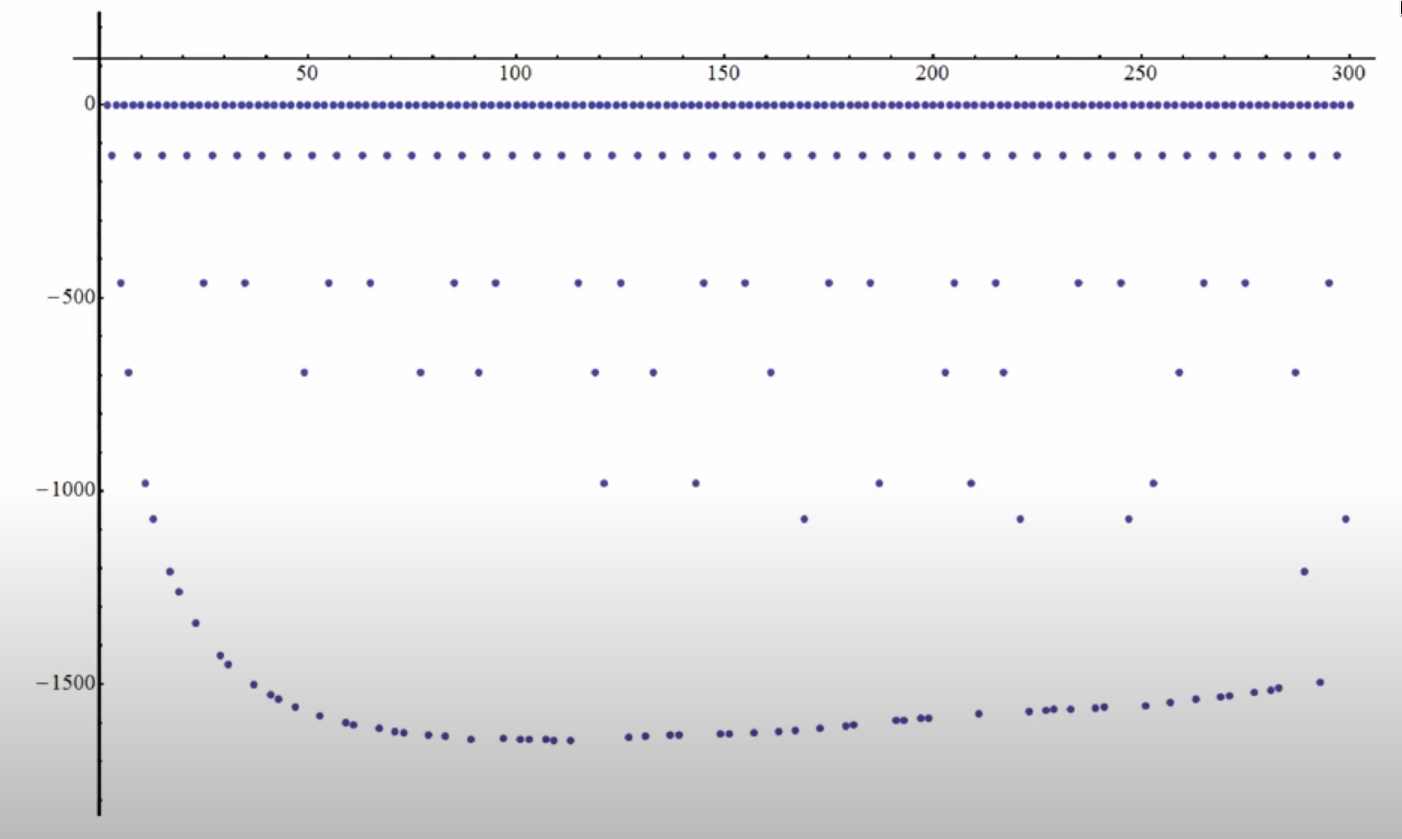
\includegraphics{./images/log.png}

\paragraph{}
Эти точки распологаются на некоторых горизонтальных уровнях.

\begin{itemize}
    \item Верхний уровень понять легко: там чётные числа, при четных числах эта функция $\approx -1$.
    То есть получается логарифм двойки.
    \item На втором уровне числа кратные трём, но не кратные двум.
    \item На третьем уровне числа, кратные пяти, но не кратные трем и пяти.
    \item ...
\end{itemize}

\paragraph{}
Но что за числа распологаются на последнем уровне? Там находятся только простые числа.
То есть мы получили РЕШЕТО ЭРАТОСФЕНА. Очень удивительно. Мы выполняли вычисления, которые никак не связаны с простыми числами и решали
СЛУ, а получили нечто похожее на решето Эратосфена. Как это доказать конечно же хороший вопрос.

\paragraph{}
Это довольно трудоёмкая деятельность. Для получения такой картинки надо решить
СЛУ из 3000 уравнений. И это очень плохая система.
Поэтому необходимо применять очень мощные компьютеры.
Однако первые 100 коэффициентов можно посчитать и на домашнем компьютере.

\end{document}
